\section{Instalación y configuración de Samba}
\label{Samba}

\subsection{Instalación}

Samba es una implementación para GNU/Linux del protocolo SMB (Server Message Block) que permite compartir recursos sobre una red TCP/IP e interconectar ordenadores Windows y Unix.

Para instalar el servidor Samba, basta con instalar el paquete \emph{samba} usando un gestor de paquetes, como apt-get o aptitude.

\begin{listing}[style=consola, numbers=none]
 # aptitude install samba
\end{listing}

El resultado obtenido será el siguiente:

\begin{SaveVerbatim}{codigo}
Leyendo lista de paquetes... Hecho
Creando árbol de dependencias
Leyendo la información de estado... Hecho
Leyendo la información de estado extendido
Inicializando el estado de los paquetes... Hecho
Construir la base de datos de etiquetas... Hecho
Se instalarán los siguiente paquetes NUEVOS:
  samba
0 paquetes actualizados, 1 nuevos instalados, 0 para eliminar y 0 sin actualizar

Necesito descargar 0B/3839kB de ficheros. Después de desempaquetar se usarán 9429kB.
Escribiendo información de estado extendido... Hecho
Preconfigurando paquetes ...
Seleccionando el paquete samba previamente no seleccionado.
(Leyendo la base de datos ...
160960 ficheros y directorios instalados actualmente.)
Desempaquetando samba (de .../samba_3.0.28a-1ubuntu4.4_i386.deb) ...
Configurando samba (3.0.28a-1ubuntu4.4) ...
 * Starting Samba daemons          [ OK ]

Leyendo lista de paquetes... Hecho
Creando árbol de dependencias
Leyendo la información de estado... Hecho
Leyendo la información de estado extendido
Inicializando el estado de los paquetes... Hecho
Escribiendo información de estado extendido... Hecho
Construir la base de datos de etiquetas... Hecho
\end{SaveVerbatim}
\respuesta{codigo}


Si se prefiere, también se pueden descargar los archivos fuente o los binarios de la distribución de la página oficial de Samba \cite{sambadownload} y posteriormente compilarlos e instalarlos siguiendo la documentación sobre la instalación \cite{sambadocu}. Existen manuales en internet que ayudan a llevar a cabo este proceso \cite{sambawiki}.

\subsubsection{Otros paquetes a instalar}

Es interesante instalar también el \textbf{demonio xinetd} (eXtended InterNET Daemon), que es una extensión más segura del servicio de Internet \emph{inetd} que viene instalado por defecto en muchas distribuciones Linux.

Estos demonios gestionan a su vez las conexiones de varios demonios, de forma que se reduce la carga del sistema al ejecutar un único demonio en lugar de todos los que gestiona.

Xinetd contiene mecanismos de control de acceso, permite habilitar los servicios de red en función del tiempo, puede limitar la cantidad de servicios que se ejecutan y contiene un sistema de protección contra escaneos de puertos, entre otras características.

\begin{listing}[style=consola, numbers=none]
# aptitude install xinetd
\end{listing}

Para instalar xinetd habrá que aceptar la desinstalación del paquete openbsd-inetd, correspondiente al demonio inetd.

\begin{SaveVerbatim}{codigo}
Se ELIMINARÁN automáticamente los siguientes paquetes:
  openbsd-inetd
Se instalarán los siguiente paquetes NUEVOS:
  xinetd
Se ELIMINARÁN los siguientes paquetes:
  openbsd-inetd
0 paquetes actualizados, 1 nuevos instalados, 1 para eliminar y 0 sin actualizar
Necesito descargar 0B/137kB de ficheros. Después de desempaquetar se usarán 242kB.
¿Quiere continuar? [Y/n/?] Y
\end{SaveVerbatim}
\respuesta{codigo}

Otro paquete que conviene instalar es \emph{swat}. Este paquete contiene la \textbf{herramienta SWAT} (Samba Web Administration Tool), que permite modificar varios parámetros de configuración del servidor Samba de forma muy sencilla a través de un navegador web.

\begin{listing}[style=consola, numbers=none]
 # aptitude install swat
\end{listing}

Para ver las opciones del comando swat (y comprobar que el paquete se ha instalado correctamente) podemos utilizar el comando \texttt{-?}.
\begin{listing}[style=consola, numbers=none]
 $ swat -?
\end{listing}

\begin{SaveVerbatim}{codigo}
 Usage: swat [OPTION...]
  -a, --disable-authentication       Disable authentication (demo mode)
  -P, --password-menu-only           Show only change password menu

Help options:
  -?, --help                         Show this help message
  --usage                            Display brief usage message

Common samba options:
  -d, --debuglevel=DEBUGLEVEL        Set debug level
  -s, --configfile=CONFIGFILE        Use alternate configuration file
  -l, --log-basename=LOGFILEBASE     Base name for log files
  -V, --version                      Print version
\end{SaveVerbatim}
\respuesta{codigo}

A continuación hay que añadir el servicio swat al archivo \texttt{services} localizado en la carpeta \texttt{/etc}.

\begin{listing}[style=consola, numbers=none]
 # echo "swat	901/tcp" >> /etc/services
\end{listing}

Lo siguiente que hay que hacer es habilitar el uso de SWAT en xinetd. Para ello se necesita conocer el directorio donde se encuentra el binario. Normalmente será uno de los siguientes:
\begin{itemize}
 \item \texttt{/usr/local/samba/bin} la localización por defecto de Samba
 \item \texttt{/usr/sbin} localización por defecto en la mayor parte de los sistemas Linux
\item \texttt{/opt/samba/bin}
\end{itemize}

Se puede comprobar la localización del binario usando el comando \emph{whereis}.

\begin{listing}[style=consola, numbers=none]
$ whereis swat
\end{listing}

\begin{SaveVerbatim}{codigo}
swat: /usr/sbin/swat /usr/share/man/man8/swat.8.gz
\end{SaveVerbatim}
\respuesta{codigo}

Una vez localizado el directorio donde se encuentra el binario de SWAT (en este caso es \texttt{/usr/sbin}),hay que editar los archivos de configuración de xinetd, que suelen ser \texttt{xinetd.conf} y otros archivos localizados en la carpeta \texttt{xinetd.d} dentro del directorio \texttt{/etc}.

El archivo \texttt{xinetd.conf} es el archivo general de configuración. Su contenido por defecto es el siguiente:

\begin{listing}
  Simple configuration file for xinetd
#
# Some defaults, and include /etc/xinetd.d/

defaults
{

# Please note that you need a log_type line to be able to use log_on_success
# and log_on_failure. The default is the following :
# log_type = SYSLOG daemon info

}

includedir /etc/xinetd.d
\end{listing}

Al final del archivo se hace una inclusión de los archivos de la carpeta \texttt{/etc/xinetd.d}, que es donde se guardan como archivos individuales los datos de configuración de los diferentes servicios.

Para habilitar SWAT,  se crea un nuevo archivo llamado \texttt{swat} dentro del directorio \texttt{/etc/xinetd.d} con el siguiente contenido:

\begin{listing}
# default: off
# description: SWAT is the Samba Web Admin Tool. Use swat \
#              to configure your Samba server. To use SWAT, \
#              connect to port 901 with your favorite web browser.
service swat
{
	port    = 901
	protocol = tcp
	socket_type     = stream
	wait    = no
	only_from = localhost
	user    = root
	server  = /usr/sbin/swat
	log_on_failure  += USERID
	disable = no
}
\end{listing}

Nótese que en al campo ``server'' se le ha asignado la localización del binario de swat.


Para que el demonio xinetd relea su configuración hay que ejecutar lo siguiente:

\begin{listing}[style=consola, numbers=none]
# /usr/bin/killall --verbose -HUP xinetd
\end{listing}

\begin{SaveVerbatim}{codigo}
xinetd(7015) eliminado con la señal 1
\end{SaveVerbatim}
\respuesta{codigo}

Una vez hecho esto, el servicio SWAT queda activado y será accesible desde un navegador accediendo a localhost por el puerto 901:

\begin{listing}[numbers=none]
http://localhost:901
\end{listing}

Para entrar a la pantalla de configuración de SWAT hay que introducir el nombre de usuario y contraseña de root del sistema.

\begin{figure}[hbt!]
 \centering
 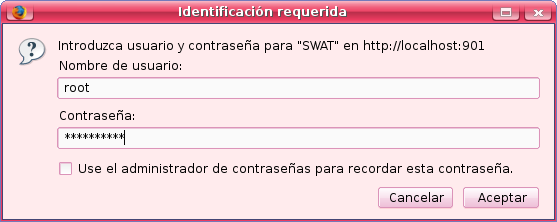
\includegraphics[width=0.95\textwidth]{Utils/swat_login.png}
 \caption{Pantalla de acceso a SWAT}
 \label{fig:swat_entrada}
\end{figure}

\newpage
\subsubsection{Resumen instalación}

\begin{enumerate}
 \item  Instalación de paquetes:
	\begin{listing}[style=consola, numbers=none]
# aptitude install samba xinetd swat
	\end{listing}

\item Añadir swat a la lista de servicios:
	\begin{listing}[style=consola, numbers=none]
# echo "swat		901/tcp" >> /etc/services
	\end{listing}

\item Crear nuevo archivo de servicio para swat
\begin{listing}[style=consola, numbers=none]
# nano /etc/xinetd.d/swat
\end{listing}

\begin{listing}[style=archivo]
# default: off
# description: SWAT is the Samba Web Admin Tool. Use swat \
#              to configure your Samba server. To use SWAT, \
#              connect to port 901 with your favorite web browser.
service swat
{
	port    = 901
	protocol = tcp
	socket_type     = stream
	wait    = no
	only_from = localhost
	user    = root
	server  = /usr/sbin/swat
	log_on_failure  += USERID
	disable = no
}
\end{listing}

\end{enumerate}
